\chapter{JOSE}
XML objects are cool and all, but are very verbose and, in some
instances, require many resources to be parsed, which is an
undesirable feature when the main focus in on IoT and embedded 
devices. This is where JSON comes in. JSON is a lightweight data
interchange format, which is also becoming the de-facto standard
for data exchange on the web. After all, XML isn't even natively
supported in mobile devices, while JSON is.

This leads to the need for industry-standard JSON-based formats for:
Security Token, Signature, Encryption and Public Key. The solutions
are: JSON Web Token (JWT), JSON Web Signature (JWS), JSON Web
Encryption (JWE) and JSON Web Key (JWK).

The design philosophy is to try to keep things as simple as possible
and to make complex things simpler without losing too many features.
The design goal was to make these things easy to use in all systems
that are already web native. For this reason, it will use compact,
URL-safe representation. URL-safe means that if an identifier of any
kind is used inside the URL, then the URL is still usable. It is known
that there are various ways to represent special character (for
example the space is substituted with \%20) so the requirement is that
any identifier used in JSON must be URL-safe because it will be
probably exchanged through a URL. The success of this is due to the
fact that these standards have been promoted and rapidly adopted by
the major internet companies (Google, Facebook, AOL, NRI, Microsoft,
\dots)

\section*{Standardization}

The following RFCs define the standards and best practices for JSON
Web technologies:
\begin{itemize}
    \item \textbf{RFC-7515}: "JSON Web Signature (JWS)".
    \item \textbf{RFC-7516}: "JSON Web Encryption (JWE)".
    \item \textbf{RFC-7517}: "JSON Web Key (JWK)".
    \item \textbf{RFC-7518}: "JSON Web Algorithms (JWA)".
    \item \textbf{RFC-7519}: "JSON Web Token (JWT)".
    \item \textbf{RFC-7797}: "JSON Web Signature (JWS) Unencoded
      Payload Option".
    \item \textbf{RFC-8725}: "JSON Web Token Best Current Practices".
    \item \textbf{RFC-7520}: "Examples of Protecting Content Using
      JSON Object Signing and Encryption (JOSE)".
\end{itemize}

\section{JSON Web Signature (JWS)}
JWS was designed to sign arbitrary content using a compact, JSON-based
representation. However, as with XML Signature, the term "signature"
in JWS is sometimes used loosely and may lead to confusion. JWS allows
for both true digital signatures and MACs. While MACs ensure
authentication and integrity, they differ from true signatures because
they rely on symmetric keys, making the roles of signer and verifier
interchangeable. In contrast, a proper digital signature clearly
distinguishes between the signer and the verifier.

JWS representation consists of three parts:
\begin{itemize}
  \item \textbf{Header}: Metadata about the signature and algorithm.
  \item \textbf{Payload}: The content being signed.
  \item \textbf{Signature}: Cryptographic signature or HMAC.
\end{itemize}

In JWS compact serialization, parts are base64url encoded and
concatenated, separated by period characters:
\begin{verbatim}
base64url(header) || '.' || base64url(payload) || '.' || base64url(signature)
\end{verbatim}

\subsection{B64 and B64url}
The specification for B64 are defined in in RFC-4648, as well as B16
and B32. Base64 encodes 6 bits at a time using an 8 bits ASCII
character, leading to a 33\% size increase (since 6 bits become 8). 
Most of the characters are allowed (A-Z, a-z, 0-9, +, /, =) except the 
padding character '=', used to make the size a multiple of 6 if
needed. Basic B64 is not URL safe because some characters(/+=) are
used in URLs. To make it URL safe, the characters are replaced with 
URL safe characters (+ becomes -, / becomes \_) and the padding 
character is removed(not added at all).

\begin{figure}[H]
  \centering
  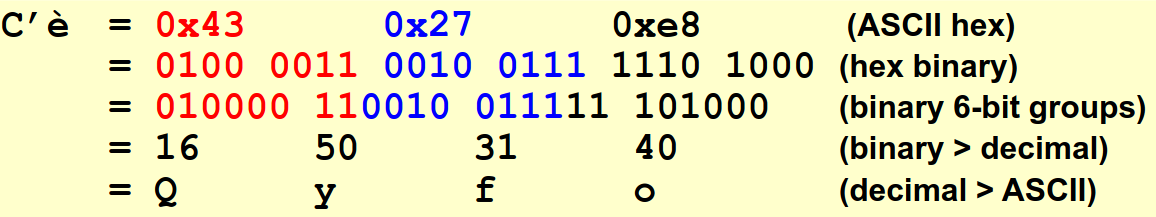
\includegraphics[width=0.8\textwidth]{img/b64 ex.png}
  \caption{An example of B64 encoding.}
  \label{fig:b64 ex}
\end{figure}

\subsection{JWS Header Parameters}

The JWS header contains various parameters to provide metadata about the signature and associated keys. These parameters include:

\begin{itemize}
    \item \textbf{"alg"}: Specifies the signature algorithm used
      (required).
    \item \textbf{"jku"}: Refers to the JSON Web Key URL.
    \item \textbf{"x5t"}: A base64url-encoded SHA-1 thumbprint of the
      DER encoding of the X.509 signature certificate.
    \item \textbf{"x5t\#S256"}: Similar to \texttt{"x5t"} but uses a
      SHA-256 thumbprint.
    \item \textbf{"x5c"}: Contains the base64-encoded DER encoding of
      the signature certificate. If a certificate chain is provided,
      it appears as a JSON array.
    \item \textbf{"x5u"}: Specifies the X.509 URL, which can be used
      to retrieve the PEM-encoded signature certificate or its chain
      (starting with the end-entity certificate and proceeding up to
      the root).
    \item \textbf{"kid"}: Represents the key identifier.
    \item \textbf{"typ"}: Indicates the type of the signed content.
\end{itemize}

\textbf{Note}: URLs referenced in the header must use an
integrity-protected channel with server authentication, such as TLS,
to ensure security.

\subsection{JSON Web Algorithm (JWA)}
JSON Web Algorithm (JWA) defines compact identifiers for algorithms
used in JWS. These include:

\begin{itemize}
    \item \textbf{"none"}: No signature (required).
    \item \textbf{"HS256"}: HMAC using SHA-256 (required).
    \item \textbf{"RS256"}: RSASSA-PKCS1-v1\_5 with SHA-256 (recommended).
    \item \textbf{"ES256"}: ECDSA with curve P-256 and SHA-256 (recommended+).
\end{itemize}

Other algorithms may be used but the ones above are the required or
the recommended ones. The recommended one are not compulsory due to an
interoperability problem: a JSON client that interacts with a JSON
server it may not have stronger implementation than the required ones.
In any case, for a complete list of JOSE parameters and supported
algorithms, refer to
\url{https://www.iana.org/assignments/jose/jose.xml}.

\subsection{JWS header and payload example}
Two examples of JWS header and payload are shown in 
Figures~\ref{fig:jws header} and~\ref{fig:jws payload}.
It's important to keep in mind that a Carriage Return Line Feed (CRLF) 
character must be present at the end of each line, except for the
last one after the closing bracket. 

The specified header is a JWT signed with HMAC SHA-256, which will be
base64url encoded.

\begin{figure}[H]
  \centering
  \begin{subfigure}[b]{0.49\textwidth}
    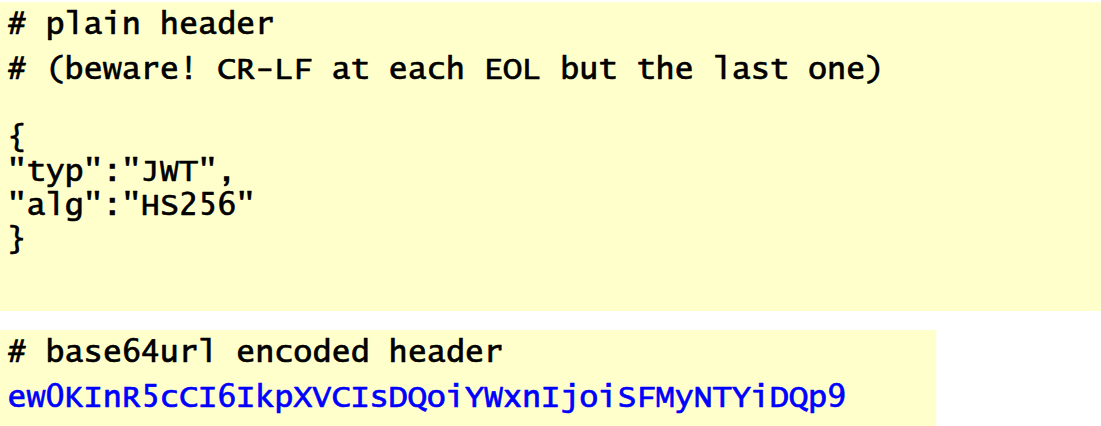
\includegraphics[width=\textwidth]{img/jws header ex.png}
    \caption{JWS header.}
    \label{fig:jws header}
  \end{subfigure}
  \begin{subfigure}[b]{0.49\textwidth}
    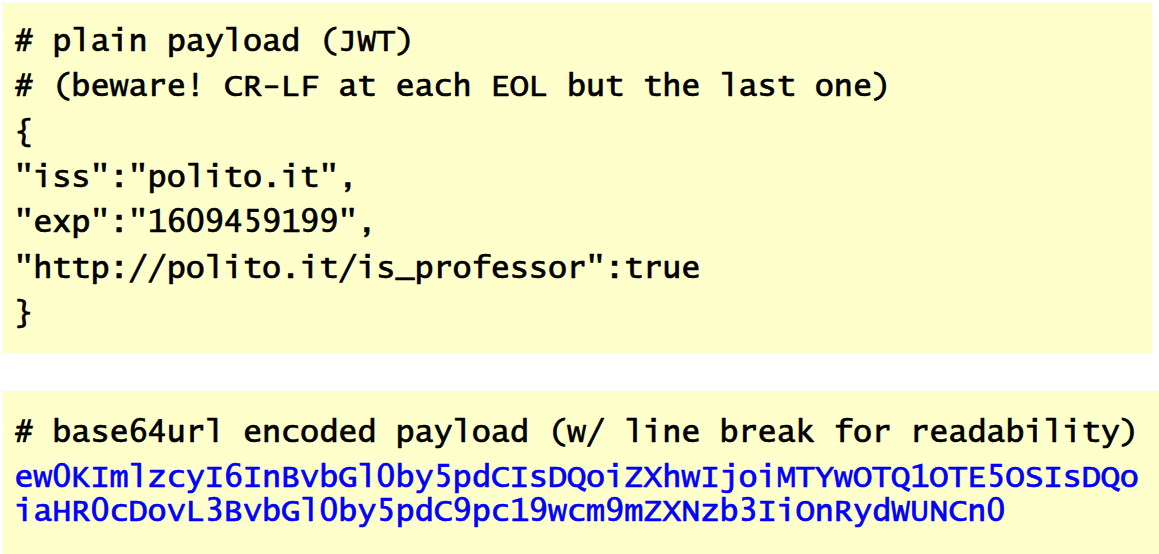
\includegraphics[width=\textwidth]{img/jws payload ex.png}
    \caption{JWS payload.}
    \label{fig:jws payload}
  \end{subfigure}
  \caption{JWS header and payload example.}
  \label{fig:jws header and payload}
\end{figure}

\subsection{JWS signature}
The signature in JWS covers both the header and the payload. This is
crucial because if the signature were to cover only the payload, the
header could be modified by an attacker. For instance, the attacker
might alter the signature algorithm or content type, potentially
causing issues with signature verification or content interpretation.

To create the signing input, the encoded header and payload are
concatenated, separated by a period (.). The resulting signature is
then generated based on this input, base64url-encoded, and appended to
the signing input after another period. This ensures the integrity of
both the header and payload.

\section{JSON Web Key (JWK)}

To perform a signature, keys are required. While the previous examples assumed that both parties already knew which key was being used, JWK (JSON Web Key) is used to explicitly represent the keys. JWK provides a standardized way to describe both asymmetric and symmetric keys.

The \texttt{kty} field specifies the key type and can have values such
as EC (Elliptic Curve, strongly recommended), RSA (required), oct
(octet sequence, also required), or OKP (Octet Key Pair).
Additionally, the kid field can be used as a key identifier, allowing
a specific key to be referenced by name.

JWK parameters vary depending on the key type and algorithm being
used. For example:
\begin{itemize}
    \item \textbf{For RSA keys:} \texttt{n} represents the modulus,
      and \texttt{e} represents the public exponent.
    \item \textbf{For AES keys:} \texttt{k} holds the key value.
\end{itemize}

\begin{figure}[H]
  \centering
  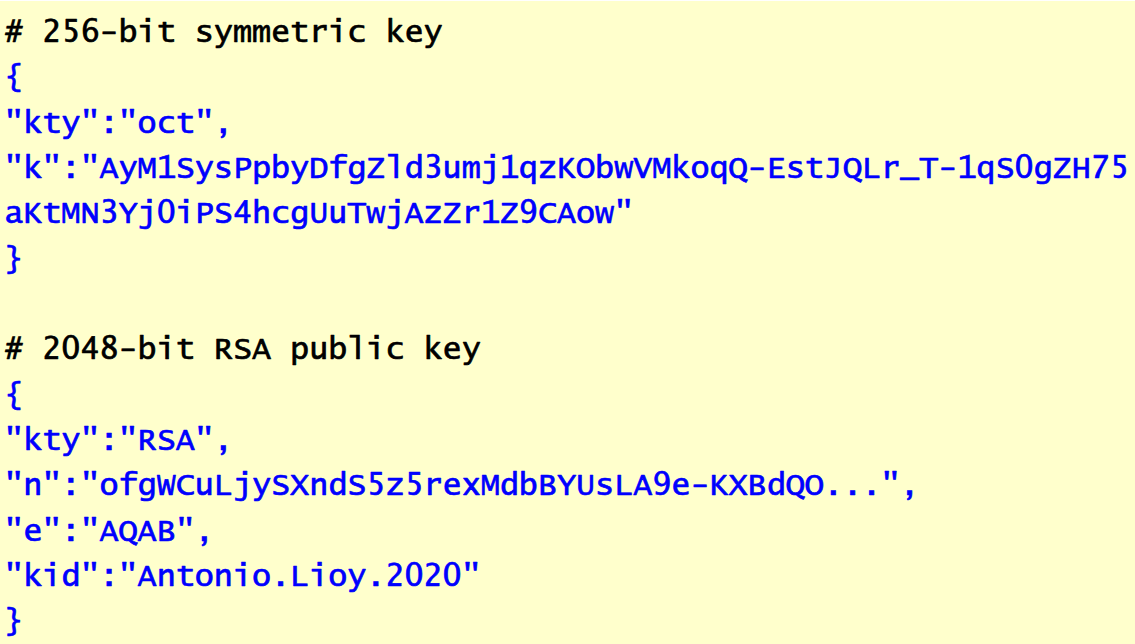
\includegraphics[width=0.7\textwidth]{img/jwk ex.png}
  \caption{Example of a JWK.}
  \label{fig:jwk ex}
\end{figure}

\section{JSON Web Encryption (JWE)}
JOSE also supports encryption through JWE, which allows arbitrary
content to be encrypted using a JSON representation. A JWE consists of
three parts: the header, the encrypted key, and the ciphertext. It can
be represented in two formats: the native JWE compact serialization
and the JWE JSON serialization. Importantly, the key is also
encrypted, so the header must specify two algorithms: one for
encrypting the key and another for encrypting the ciphertext.

\subsection{JWE Header Parameters}

The JWE (JSON Web Encryption) header contains several important
parameters:

\begin{itemize}
    \item \texttt{alg} = The key encryption algorithm, used to protect
      the Content Encryption Key (CEK).
    \item \texttt{enc} = The content encryption algorithm, used to
      encrypt the actual content.
    \item Key identification parameters (similar to those in JWS):
    \begin{itemize}
        \item \texttt{jku} = The URL of the JSON Web Key.
        \item \texttt{x5t} = The SHA-1 thumbprint of the X.509
          certificate.
        \item \texttt{x5t\#S256} = The SHA-256 thumbprint of the X.509
          certificate.
        \item \texttt{x5c} = The X.509 certificate.
        \item \texttt{x5u} = The URL of the X.509 certificate.
        \item \texttt{kid} = The key identifier.
    \end{itemize}
\end{itemize}

\subsection{JWE Compact Serialization}
As previously mentioned, JWE can be represented in two formats. The 
compact serialization format is similar to JWS, with the header, 
encrypted key, and ciphertext concatenated and separated by periods,
but it also has more parts:
\begin{verbatim}
base64url(header) || '.' || base64url(encrypted CEK) || '.' ||
base64url(iv) || '.' || base64url(ciphertext) || '.' || base64url(auth
tag)
\end{verbatim}


There’s only one recipient (one of the limits) which means that it is
not something that can be decrypted by many recipients (in PKCS\#7
there was the possibility for both signatures to have various signers
and encryption to have keys encrypted for several recipients), because
JSON is thought to be exchanged between one client and one server.
There are also no unprotected headers and no associated data (so the
tag is computed on everything).

\subsection{JWE JSON Serialization}

This is the second format for JWE. JWE JSON serialization represents
encrypted content as a JSON object with the following top-level
members (all optional except for the ciphertext):

\begin{itemize}
    \item \texttt{"protected"}: Integrity-protected headers.
    \item \texttt{"unprotected"}: Other (unprotected) headers.
    \item \texttt{"iv"}: Initialization vector.
    \item \texttt{"aad"}: Additional authenticated data.
    \item \texttt{"ciphertext"}: The actual encrypted content.
    \item \texttt{"tag"}: Authentication tag.
    \item \texttt{"recipients"}: An array of JSON objects identifying
      each recipient and providing the CEK encrypted with their public
      key.
    \item \texttt{header \{alg, kid\}}: Algorithm and key identifier
      for encryption.
    \item \texttt{encrypted\_key}: The encrypted content encryption
      key.
\end{itemize}
An example of JWE JSON serialization is shown in 
Figure~\ref{fig:jwe json ex}.
The example demonstrates the structure of the protected and
unprotected headers, with the unprotected header containing the key
identifier. The "recipients" field includes the header specifying the
algorithm and the key identifier, followed by the encrypted key, which
is encrypted using the public key indicated by the identifier. In the
case of the second recipient, the algorithm "a128kw" refers to
AES-128-KW (Key Wrap), where the symmetric key is encrypted using
another symmetric key. A previous agreement has been made about the
key identified by number 7, and then the key is encrypted.

Next, the structure includes the initialization vector, the actual
ciphertext, and the authentication tag. Notably, the algorithm used is
not explicitly specified, as it is optional. In this example, it is
assumed that the encryption algorithm declared externally was
"A128CBC-HS256" (AES 128 CBC with HMAC SHA256 for the authentication
tag). While the name implies encryption, the format supports both
encryption and message authentication. It's possible to use the same
format by specifying null for encryption and using only the
authentication portion, though JWS would be preferred for that
scenario. The standard format avoids using encryption, followed by
re-encapsulation in a signature, in cases where both encryption and
authentication are required.

\begin{figure}[H]
  \centering
  \includegraphics[width=0.7\textwidth]{img/jwe json serialization
  ex.png}
  \caption{Example of a JWE JSON serialization.}
  \label{fig:jwe json ex}
\end{figure}

